\documentclass[sigplan,anonymous,review,nonacm]{acmart}
\usepackage{amsmath,amssymb,amsfonts}
\usepackage{booktabs}
\usepackage{graphicx}
\usepackage{xcolor}
\usepackage{microtype}
\usepackage{placeins}
\usepackage{tikz}
\usetikzlibrary{arrows.meta,positioning}
\graphicspath{{figures/}}

\title{Beyond Byte Counts: What Determines KV-Cache Quality and Decode Performance?}

\begin{document}

% ==================================================================
\begin{abstract}
KV-cache methods are usually compared by how many bits they store or how few tokens
they attend, but neither quantity determines performance by itself. Compression
changes the representation kept in memory; sparse selection adds a scoring pass that
ranks cached keys before attention. Published comparisons often vary the value-cache
precision, recent-token policy, scoring representation, and access pattern together,
making it difficult to identify why one method wins. We re-evaluate representative
compression and selection mechanisms under matched conditions and profile the
resulting kernels on an RTX~4000 Ada. Three mechanisms explain the observed rankings.
First, in a five-seed compression ablation, changing the value representation shifts
PPL by 4.80--5.72, whereas the tested key configurations span 0.89 within the FP8
value column. Second, selection granularity matters more than code sophistication in
the observed panel: scalar int4 and product-quantized keys give similar selections at
the same 32-byte scoring cost, whereas our page-level implementation requires a
larger retained-key budget. Third, fewer bytes do not guarantee lower latency. Our
packed int4 and int2 scoring kernels lose to fp8 at the measured point despite moving
fewer score bytes. We also identify a numerical failure in which bf16 score
accumulation mis-ranks keys and fp16 overflows. The resulting design rule is to
evaluate storage, scoring, and attention as separate stages, then compose them only
after validating both quality and realized kernels.
\end{abstract}
\maketitle

% ==================================================================
\section{Introduction}
Long-context autoregressive decoding repeatedly reads the key--value (KV) cache, which
stores attention keys and values for every previous token and every transformer
layer. As the context and batch grow, this cache consumes both device memory and
memory bandwidth. Compression methods reduce the number of stored bits, while sparse
attention methods read values for only a selected subset of tokens. Because both
approaches reduce nominal bytes, they are often presented on a common efficiency
axis. That comparison hides a basic systems distinction: compression reduces
\emph{storage}, whereas selection introduces work to decide which entries to read.

This distinction creates a recurring mismatch between theoretical savings and
measured behavior. A two-bit key representation can occupy one quarter of an fp8 key,
yet take longer to score if the GPU must unpack and convert it. A selector can read
few values, yet still scan every key and run a global top-$k$ operation. Likewise, a
key quantizer can appear more accurate simply because it is paired with a more
accurate value cache. Although byte counts suggest a single ranking, the actual
quality, capacity, and latency rankings are set by different stages of the decode
pipeline.

We isolate those stages under a matched protocol. Every selector receives the same
retained-key budget, recent-token window, and bf16 attention cache. Compression
methods are compared at a common value precision. Latency measurements include the
score, top-$k$, and gather operations inside a CUDA graph, and controlled kernels are
checked against reference attention before profiling. The study covers two model
families, Qwen2.5 models from 0.5B to 7B, Llama-3.2-3B, Wikitext-2 and PG19, and
contexts from 8K to 32K.

The contribution is a controlled diagnosis rather than a new KV-cache algorithm.
Prior benchmarks have already shown that nominal compression ratios do not determine
deployment performance, and prior sparse--quantized systems have shown that the two
mechanisms interact. Our narrower contribution is to localize each observed ranking
to separately controlled stages under a protocol that varies one stage at a time:
\begin{itemize}
\setlength{\itemsep}{1pt}\setlength{\topsep}{3pt}\setlength{\leftmargin}{1.2em}
\item We independently control value-cache precision, scoring representation,
selection unit, and score accumulation, revealing cross-axis effects hidden by an
aggregate compression ratio.
\item We identify a low-precision failure of the exact-key ranking oracle,
then specify finite-score and ranking-agreement checks needed to validate it.
\item We connect scoring representation to realized execution, showing why packed
low-bit scoring loses its nominal byte advantage at the measured Ada operating point.
\end{itemize}

% ==================================================================
\section{Background and Related Work}

\subsection{The decode path and its three representations}
At decode step $t$, each attention head forms a query $q_t$ and scores every cached
key $k_i$ using $q_t^\top k_i$. Dense attention normalizes these scores and combines
all cached values $v_i$. A sparse selector instead estimates the scores, retains a
top-$k$ subset, gathers the corresponding keys and values, and performs attention on
that subset. Here, $k$ denotes a \emph{percentage of historical keys}, not the number
of neighbors; a 5\% budget at a 16K context retains roughly 819 historical positions,
plus the fixed recent window used in our protocol.

Figure~\ref{fig:pipeline} separates three representations that are often conflated.
The \emph{stored cache} determines memory capacity. The \emph{scoring representation}
is read for every cached key and determines the cost and accuracy of selection. The
\emph{attention representation} supplies the selected keys and values and determines
the final attention error. One method may use the same representation for all three;
our controlled experiments deliberately separate them.

\begin{figure*}[t]
\centering
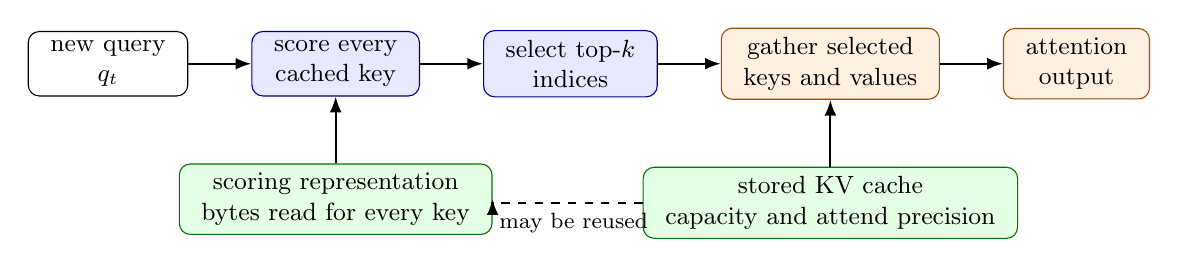
\begin{tikzpicture}[
  node distance=0.75cm and 0.8cm,
  box/.style={draw,rounded corners,minimum height=0.8cm,align=center,font=\small,inner xsep=8pt},
  select/.style={box,fill=blue!9,draw=blue!55!black},
  store/.style={box,fill=green!10,draw=green!45!black},
  attend/.style={box,fill=orange!12,draw=orange!60!black},
  arrow/.style={-{Latex[length=2mm]},thick}
]
\node[box] (query) {new query\\$q_t$};
\node[select,right=of query] (score) {score every\\cached key};
\node[select,right=of score] (topk) {select top-$k$\\indices};
\node[attend,right=of topk] (gather) {gather selected\\keys and values};
\node[attend,right=of gather] (attention) {attention\\output};
\node[store,below=0.85cm of score] (scorecache) {scoring representation\\bytes read for every key};
\node[store,below=0.85cm of gather] (attendcache) {stored KV cache\\capacity and attend precision};
\draw[arrow] (query) -- (score);
\draw[arrow] (score) -- (topk);
\draw[arrow] (topk) -- (gather);
\draw[arrow] (gather) -- (attention);
\draw[arrow] (scorecache) -- (score);
\draw[arrow] (attendcache) -- (gather);
\draw[arrow,dashed] (attendcache.west) -| node[pos=0.23,below,font=\footnotesize] {may be reused} (scorecache.east);
\end{tikzpicture}
\Description{A flow diagram of a sparse KV-cache decode step. A new query flows into a
box that scores every cached key, which flows into a box that selects top-k indices,
which flows into a box that gathers the selected keys and values, which flows into the
final attention output. Below the scoring box, a green box labeled "scoring
representation: bytes read for every key" feeds into it. Below the gather box, a
second green box labeled "stored KV cache: capacity and attend precision" feeds into
it, with a dashed arrow indicating the stored cache representation may be reused as
the scoring representation.}
\caption{A sparse KV-cache decode step. Selection (blue) scans a scoring
representation for every historical key, runs top-$k$, and returns indices. Attention
(orange) then gathers only the selected entries from the stored KV cache (green).
Compression primarily changes stored capacity and decode work; selection primarily
changes the score scan and the number of gathered values.}
\label{fig:pipeline}
\end{figure*}

\subsection{Prior methods and where this study differs}
KIVI~\cite{liu2024kivi} stores integer keys and values with group metadata and decodes
them using a packed-integer kernel. KVQuant~\cite{hooper2024kvquant} combines
non-uniform quantization with explicit outlier channels. Product quantization (PQ)
represents a key by codebook indices; PQCache~\cite{zhang2025pqcache} reuses those
indices to estimate query--key scores. Self-Indexing KVCache~\cite{yang2026selfindexing}
similarly predicts sparse attention from a sign-based vector code. These methods can
reduce storage, provide a scoring proxy, or do both. KVTuner~\cite{li2025kvtuner}
finds that key and value caches have different, layer-dependent quantization
sensitivity and often allocates more bits to keys. Our value-cache ablation does not
claim the opposite universally: it shows that, for the particular matched key tier
and value formats evaluated here, changing the value representation is the dominant
source of the reported PPL difference.

Selection methods differ in \emph{what unit they rank}. Per-key methods score each
token separately. Quest~\cite{tang2024quest} scores page-level bounds, so selecting
one relevant token also retains its neighbors. SparQ~\cite{ribar2024sparq} scores
keys using only the largest query channels. H2O~\cite{zhang2023h2o} and
SnapKV~\cite{li2024snapkv} evict entries using accumulated or observation-window
attention, avoiding a full score scan at decode time but permanently discarding
tokens. TokenSelect~\cite{wu2025tokenselect} previously established the value of
fine-grained token selection, while MagicPIG~\cite{chen2025magicpig} shows that even
exact top-$k$ can be a poor approximation to dense attention on some tasks. We do not
present token-level selection as new or treat exact top-$k$ as a dense-attention
oracle. It is only the best ranking reference at the same sparse budget; our question
is whether representation error or decision granularity moves a selector away from
that reference.

Q-Hitter~\cite{zhang2024qhitter} is the closest precedent for isolating these stages:
it derives a selected set from quantized scores, then evaluates that set with
full-precision KV entries to expose attention shift. We adopt the same essential
control but ask a different question, comparing several scalar, product-quantized,
and sign-based scoring representations at matched retained-key budgets and separating
their score traffic from the precision of the attended cache. LServe~\cite{yang2025lserve}
instead demonstrates a deployable co-design that fuses block sparsity and KV
quantization. Our controlled kernels are not proposed as a competing serving system;
they isolate when the scoring representation itself changes the bottleneck.

Finally, prior evaluations cover broad method and workload tradeoffs.
Yuan et al.~\cite{yuan2024longctx} compare more than ten long-context approaches,
SCBench~\cite{li2025scbench} evaluates the KV-cache lifecycle under shared contexts,
and Rethinking KV-Cache Compression~\cite{wei2025rethinking} examines throughput,
response length, and failure cases in serving. A recent workload-aware
benchmark~\cite{agrawal2026benchmarking} likewise finds that compression ratio alone
poorly predicts end-to-end behavior. We therefore do not claim the first fair
benchmark or the first size--performance mismatch. We provide a finer stage-level
decomposition: fixed budgets and attention precision for quality, followed by
stage-level profiling that attributes the remaining latency to score, ranking,
gather, or decode kernels.

\begin{table*}[t]
\centering\small
\caption{Closest-work boundary. This paper is a controlled characterization, not a
new quantizer, selector, or production serving system.}
\label{tab:closest-work}
\begin{tabular}{p{0.19\textwidth}p{0.30\textwidth}p{0.43\textwidth}}
\toprule
Closest line of work & Shared ground & Distinction and non-claim here \\
\midrule
KIVI~\cite{liu2024kivi}, KVQuant~\cite{hooper2024kvquant},
PQCache~\cite{zhang2025pqcache}, Self-Indexing KVCache~\cite{yang2026selfindexing}
& Quantized KV representations and approximate score keys.
& We do not propose a codec. We hold representation, attended-cache precision, and
budget apart; report raw quality/capacity/latency evidence; and characterize the
measured packed-score path. \\
Quest~\cite{tang2024quest}, SparQ~\cite{ribar2024sparq},
H2O~\cite{zhang2023h2o}, SnapKV~\cite{li2024snapkv}, TokenSelect~\cite{wu2025tokenselect}
& Sparse or eviction-based KV reduction and token/page decisions.
& We do not claim a new selection policy. We compare decision granularity under a
matched budget and distinguish a score scan, top-$k$, and selected-value gather. \\
Q-Hitter~\cite{zhang2024qhitter} and MagicPIG~\cite{chen2025magicpig}
& Decoupling approximate selection from exact attention; limits of top-$k$ sparsity.
& We extend the control across scoring representations and attended-cache formats,
and make exact top-$k$ only a same-budget ranking reference, not a dense-attention
oracle. \\
Long-context/KV benchmarks~\cite{yuan2024longctx,li2025scbench} and
Rethinking KV-Cache Compression~\cite{wei2025rethinking}
& Broad method/workload evaluation and the observation that compression ratio alone
does not predict serving behavior.
& We do not claim the first benchmark. The added evidence is a per-stage decode
characterization, controlled null result for the numerical mechanism, and released
per-observation traces for the stated operating point. \\
LServe~\cite{yang2025lserve}
& Joint sparsity--quantization systems and end-to-end performance goals.
& Our kernels are diagnostic controls, not a competing optimized serving stack;
conclusions are intentionally limited to the evaluated implementation and Ada GPU. \\
\bottomrule
\end{tabular}
\end{table*}

\subsection{How to read the measurements}
Perplexity (PPL) is the exponential of average token negative log-likelihood; lower is
better. Each quality table states its dense or full-precision reference, and
$\Delta$PPL means the increase relative to that reference. The selection budget is
the percentage of historical keys retained. ``B/key'' counts bytes read \emph{per key
head} to rank one cached position; it is not the total KV-cache size. The ``exact
selector'' computes scores from unquantized keys but still attends only to its top-$k$
subset, so it is an oracle for ranking quality rather than dense attention. Latency is
wall-clock time per decode step at the stated tensor shape, while achieved bandwidth
is reported as a percentage of the GPU's 360\,GB/s peak. These definitions keep
storage, selection, and attention costs on separate axes.

% ==================================================================
\section{Methodology}

\subsection{Quality evaluation}
We evaluate Qwen2.5-0.5B/1.5B/3B/7B and Llama-3.2-3B, with attention head dimensions
64 and 128, on Wikitext-2-raw and PG19. Long-context PPL is computed on the final 512
positions of contiguous 8K, 16K, or 32K windows, where each prediction has the
longest available history. We apply the model's language-model head only to those tail
states to avoid materializing full-sequence logits. Synthetic Needle-in-a-Haystack
(NIAH) retrieval separately tests whether a selector can retain a rare relevant key.

For the selection study, every method ranks the same keys, keeps
$k\in\{1,2,5,10\}\%$, and always includes the most recent 32 tokens. Selected
entries are read from the same exact bf16 key/value cache, so PPL differences measure
selection rather than attention quantization. Scoring costs are charged from the
representation actually scanned: exact keys scored in fp32 use $2D$ bytes, fp8 uses $D$, int4
and PQ-LUT use $D/2$, sign-VQ uses approximately $3D/8$, and int2 uses $D/4$.
Unless explicitly varied, dot products accumulate in fp32. The compression ablation
instead holds the key tier fixed while varying the value representation, then holds
the value representation fixed when comparing key quantizers.

\subsection{Latency, profiling, and validation}
System measurements use an RTX~4000 Ada with 20\,GB memory at $B{=}32$,
$S{=}16$K, $D{=}128$, $H_q{=}64$, and $H_k{=}8$. Each latency is measured from
200 CUDA-graph replays after 20 warmups; scoring, top-$k$, and gather all execute
inside the graph. The tensor shapes match a large grouped-query-attention layer, while
quality experiments use the real models above. Measured achieved bandwidth and the
stage decomposition distinguish kernels limited primarily by data movement from paths
where unpacking or arithmetic dominates.

The original operating-point profile is complemented by two additional robustness
panels on the same device. The first repeats the complete sparse decode path (score,
top-$k$, and gather) over 15 independently captured CUDA graphs at 8K and 16K
contexts and 1, 5, and 10\% budgets; each capture is timed over 100 replays. The
second isolates only the all-key score kernel while sweeping $S\in\{8,16\}$K and
$D\in\{64,128,256\}$ at the same grouped-query shape. We report medians and 2.5th--
97.5th percentile ranges of those independent captures, not a spurious precision from
a single graph replay.

KIVI uses its official CUDA kernel. Other controlled kernels are checked against
reference attention with at most $10^{-2}$ error before timing. The evidence bundle
contains per-window or per-trial observations, environment metadata, and
consolidation scripts. This lets the main paper explain regimes and mechanisms without
treating an aggregate as its only evidence.

% ==================================================================
\section{Results}

\subsection{Value precision sets the quality scale}
The value cache is the first variable to control because it can overwhelm differences
among key representations. Table~\ref{tab:value} holds the tested key configurations
fixed while changing only the value cache. Moving from the 2-bpw PQ value cache to
FP8 changes PPL by 4.80--5.72 across the five rows. By comparison, the five key
configurations span 0.89 PPL within the FP8 column. In this protocol, a comparison
that changes both key method and value precision cannot assign its quality gain to the
key method.

\begin{table}[t]
\centering\footnotesize\setlength{\tabcolsep}{3pt}
\caption{PPL when the key configuration and value precision are varied separately
(Qwen2.5-0.5B, Wikitext-2, five seeds). Lower is better. The observed value-mode
gaps are 4.80--5.72 PPL, versus a 0.89-PPL span within the FP8 column.}
\label{tab:value}
\resizebox{\columnwidth}{!}{\begin{tabular}{lcc}
\toprule
\textbf{Key configuration} & \textbf{PQ value (2\,bpw)} & \textbf{FP8 value (8\,bpw)} \\
\midrule
PQ (No Rot.) & 24.21$\pm$0.64 & 19.42$\pm$0.26 \\
Rotated PQ & 25.39$\pm$0.80 & 20.13$\pm$0.27 \\
Rotated PQ + calibration & 26.02$\pm$0.69 & 20.31$\pm$0.51 \\
\quad + sign-pattern selection & 25.25$\pm$0.47 & 19.92$\pm$0.09 \\
\textbf{\quad + outlier isolation} & \textbf{25.26$\pm$0.70} & \textbf{19.97$\pm$0.30} \\
\bottomrule
\end{tabular}
}
\end{table}

Once the attention cache is fixed, the key code has a much smaller effect on
selection. Figure~\ref{fig:budget} shows two clear regimes. Per-key selectors approach
the dense reference by a 5\% budget, whereas page selection and eviction remain
visibly above it. Within the per-key group, fp8, PQ-LUT, and int4 follow nearly the
same curve despite using 64, 32, and 32 scoring bytes per key, respectively. Sign-VQ
and int2 save additional bytes but incur a larger quality gap.

\begin{figure*}[t]
\centering
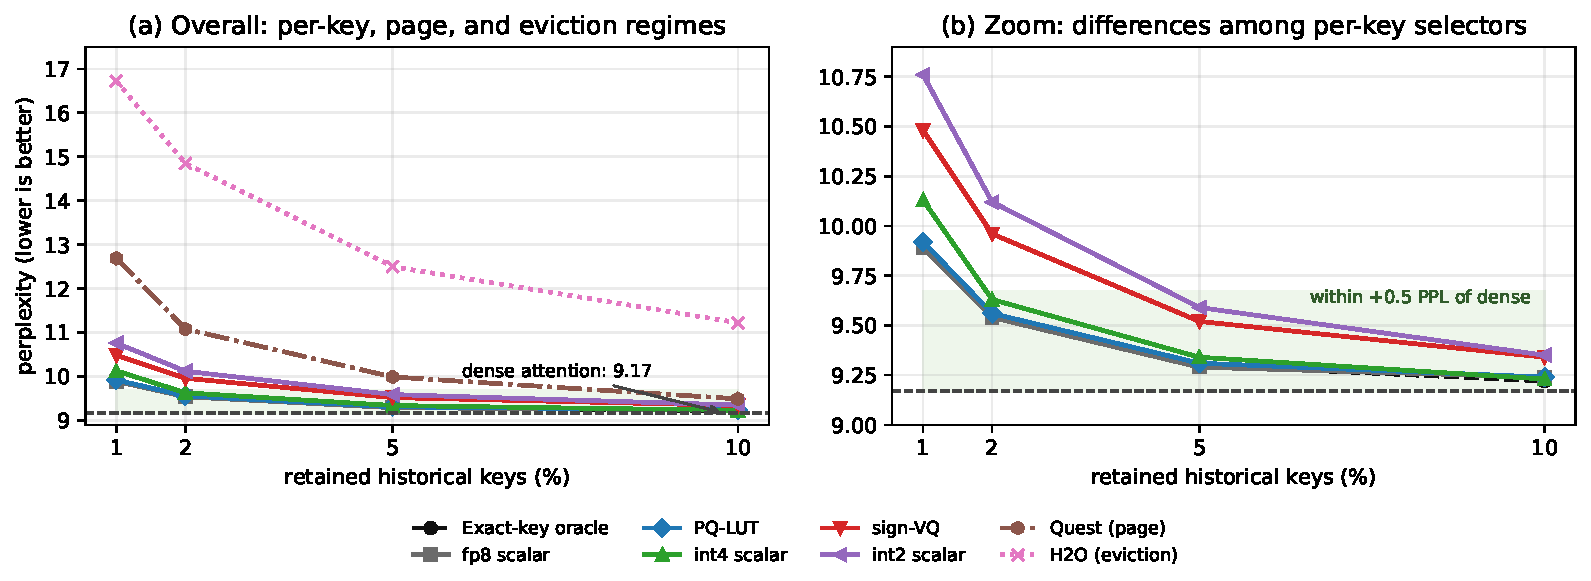
\includegraphics[width=0.97\textwidth]{fig_study_budget_readable.pdf}
\Description{Two line charts of perplexity versus retained-key budget for Qwen2.5-0.5B
at 16K context. The left panel shows exact-key, fp8, PQ-LUT, int4, sign-VQ, and int2
per-key selectors clustering near the dense-attention reference as budget increases,
while Quest (page) and H2O (eviction) remain well above it. The right panel zooms into
the per-key selectors, which converge within 0.5 PPL of dense attention by a 5--10\%
budget.}
\caption{Selection quality as the retained-key budget increases
(Qwen2.5-0.5B, 16K context). The vertical axis is PPL, so lower is better; the dashed
line is dense attention using every key. ``Exact'' is the best ranking available at
the same sparse budget, not dense attention. Per-key methods form the lower cluster
and enter the near-dense regime around 5--10\%, while page selection and eviction
require more retained context. All methods use the same 32-token recent window and
the same bf16 attention cache.}
\label{fig:budget}
\end{figure*}

Table~\ref{tab:selection} makes the representative 5\% operating point explicit.
The PPL column is the measured model perplexity; $\Delta$PPL subtracts the dense
reference of 9.17. PQ-LUT and int4 have the same 32-byte score read and differ by
0.03 PPL. Quest also has a small amortized score representation, but its page-level
unit produces a 0.82 PPL gap. The result is not that one scalar format always wins;
it is that code sophistication does not explain the dominant quality separation once
attention precision and recent context are matched.

\begin{table*}[t]
\centering\small\setlength{\tabcolsep}{8pt}
\caption{Representative selection operating point at a 5\% budget
(Qwen2.5-0.5B, 16K context, dense PPL 9.17). ``Score representation'' is what the
selector scans for every historical key; ``selection unit'' states whether it ranks
individual keys, pages, or performs eviction. Lower PPL and $\Delta$PPL are better.}
\label{tab:selection}
\begin{tabular}{l c c r r}
\toprule
selector & score representation & selection unit & PPL & $\Delta$PPL \\
\midrule
exact keys & fp32 score, 128 B/key & key & 9.30 & +0.13 \\
fp8 scalar & fp8, 64 B/key & key & 9.29 & +0.12 \\
PQ-LUT & PQ indices, 32 B/key & key & 9.31 & +0.14 \\
int4 scalar & int4, 32 B/key & key & 9.34 & +0.17 \\
sign-VQ & sign-VQ, 24 B/key & key & 9.52 & +0.35 \\
int2 scalar & int2, 16 B/key & key & 9.59 & +0.42 \\
Quest & bounds, 16 B/key & page & 9.99 & +0.82 \\
H2O & no per-step scan & eviction & 12.50 & +3.33 \\
\bottomrule
\end{tabular}

\end{table*}

\subsection{Selection granularity explains the largest quality gap}
The page result persists when retrieval, rather than average language-model loss, is
isolated. At a 1\% NIAH budget, exact, PQ-LUT, and int4 per-key selectors retrieve
97--98\% of needles, while our page-based Quest implementation retrieves 20\%.
Changing Quest's page size from 64 to 16 improves PPL monotonically, but the finest
tested page still trails every per-key code. The mechanism is direct: a relevant key
causes the entire page to consume budget, so unrelated neighbors displace other useful
keys. H2O and SnapKV face a different limitation: once a key is evicted, a later query
cannot recover it. Their 16K PPL remains above the dense reference at every tested
budget.

This result also clarifies how to interpret scoring bytes. Quest reads only 16 bytes
of page bounds per key after amortization, but those bytes describe a coarser decision
unit than 16 bytes of per-key int2 scores. Equal byte counts therefore do not imply
equal information or equal selected sets. For quality comparisons, scoring cost must
be reported together with the unit being selected.

Table~\ref{tab:retrieval_pages} makes the two controls concrete. The NIAH intervals
are paired-trial bootstrap intervals over 100 retrieval cases, rather than a single
aggregate score. They show that the retrieval difference at $1\%$ is not a marginal
PPL effect. The page sweep also identifies a continuous tradeoff within the same
mechanism: smaller pages improve the tested PPL monotonically, but do not remove the
gap at the tested budgets. These controls support a granularity explanation without
claiming that every page-based selector behaves identically.

\begin{table*}[t]
\centering\small
\caption{Two controls for selection granularity (Qwen2.5-0.5B, 16K). Left: NIAH
retrieval rate with 95\% paired bootstrap intervals. Right: PPL of the same Quest
implementation as its page size changes (dense PPL 9.17).}
\label{tab:retrieval_pages}
\begin{minipage}[t]{0.47\textwidth}
\centering\textbf{NIAH retrieval}\\[1pt]
\resizebox{\linewidth}{!}{\begin{tabular}{l c c c}
\toprule
selector & $k{=}0.5\%$ & $k{=}1\%$ & $k{=}2\%$ \\
\midrule
exact & 0.96 [0.90,0.98] & 0.97 [0.92,0.99] & 0.98 [0.93,0.99] \\
PQ-LUT & 0.95 [0.89,0.98] & 0.97 [0.92,0.99] & 0.98 [0.93,0.99] \\
int4 scalar & 0.93 [0.86,0.97] & 0.98 [0.93,0.99] & 0.98 [0.93,0.99] \\
Quest & 0.00 [0.00,0.04] & 0.20 [0.13,0.29] & 0.33 [0.25,0.43] \\
\bottomrule
\end{tabular}
}
\end{minipage}\hfill
\begin{minipage}[t]{0.43\textwidth}
\centering\textbf{Quest page-size}\\[-1pt]
\textbf{control}\\[1pt]
\resizebox{\linewidth}{!}{\begin{tabular}{l r r r r}
\toprule
Quest page & $k{=}1\%$ & $k{=}2\%$ & $k{=}5\%$ & $k{=}10\%$ \\
\midrule
page$=$16 & 12.69 & 11.08 & 9.99 & 9.49 \\
page$=$32 & 13.30 & 11.66 & 10.16 & 9.58 \\
page$=$64 & 15.00 & 12.20 & 10.63 & 9.88 \\
\bottomrule
\end{tabular}
}
\end{minipage}
\end{table*}

\subsection{The ranking oracle can fail numerically}
The matched experiment exposed a measurement failure before it exposed a method
difference. On Qwen2.5-1.5B, a quantized selector initially appeared to outperform
the unquantized-key oracle. Score-range, nonfinite-count, and top-$k$-agreement checks
traced the anomaly to accumulation precision. At a 10\% budget, the oracle degrades
from 6.73 PPL in fp32 to 8.01 in bf16, while the dense reference is 6.71. The model
does contain large key channels ($|k|\!\approx\!326$), so we tested the concrete
hypothesis that they alone cause the instability: we capped only selection-key
channels at 256, 128, and 64, while leaving the exact post-selection attention keys
and values unchanged. The corresponding bf16 PPLs are 7.86, 8.07, and 7.91. Clipping
therefore does \emph{not} restore fp32-quality ranking. The evidence supports a
broader low-precision ranking instability, not a single-channel causal explanation.

Fp16 has more mantissa bits but a smaller exponent range; it produces NaN PPL at the
tested $k{=}10\%$ budget. The present measurements identify this as an arithmetic
failure mode, but do not isolate the exact operation at which non-finite values arise.
The other tested models change by at most 0.02 PPL across formats, which explains why
the bug is easy to miss. We consequently use fp32 accumulation for all selection
scores. An ``exact'' selector is only a valid oracle after finite-score and ranking
agreement checks establish that its arithmetic is reliable.

\subsection{Fewer score bytes can increase decode latency}
The score representation is scanned for every key, so low-bit packing appears to be
the natural way to accelerate sparse decode. The profile in
Figure~\ref{fig:profiling} shows why that expectation fails here. Random, contiguous,
and paged gathers each sustain about 76\% of peak bandwidth, a contiguous bf16 stream
reaches 49\%, and KIVI's packed-integer decode reaches 33\%. Thus a byte does not have
a fixed time cost: at this operating point, the gather kernels process bytes about
2.3$\times$ faster than the packed KIVI path.

The sparse decomposition identifies a second bottleneck. The score pass reads every
key regardless of the retained budget, top-$k$ contributes an approximately 2.5\,ms
ranking cost, and only the final gather shrinks substantially with $k$. Packing int4
or int2 reduces nominal score-key storage, but it does not reduce the work of this
implementation proportionally. For every reconstructed key scalar, the packed kernel
performs a shift, mask, type conversion, scale/zero reconstruction, multiply, and add
before the fp32 dot product. Its vectorized pointer expressions also repeat each
packed-byte address for every value encoded in that byte and repeat group-metadata
addresses for the 32 values in a quantization group. The Triton source path thus has
substantially more scalar reconstruction work and less regular effective traffic than
the fp8 load--convert--dot path. At a 5\% budget, int2 scoring is 1.8$\times$ slower
than fp8 and int4 is 2.7$\times$ slower (Table~\ref{tab:latency}). This is a
source-level mechanism consistent with the measurements; we do not claim a specific
Ada issue-port or instruction-stall attribution without hardware counters.
The controlled reconstruction ablation at the primary 16K/$D{=}128$ shape makes the
software contribution explicit: int2 rises from 2.52 ms for the packed-load-only
stage to 2.74 ms after bit extraction, 3.25 ms after dequantization, and 8.37 ms
for the full dot-product path. Int4's packed-load stage is already 9.89 ms and its
full path is 14.90 ms. These stage timings establish added reconstruction work in
this implementation; they are not hardware-counter measurements of issue pressure.

The gather result also has a useful boundary. Random and paged selected-value gathers
reach 70--80\% of peak over the sparse budgets at $D{=}128$, where one bf16 value row is 256 bytes. In the
same kernel with a full-cache sweep, random gathering is only 51--62\% as efficient
as contiguous gathering for 16--64-byte rows, but reaches 98--100\% for rows of 128
bytes or more. Thus the result is not that arbitrary noncontiguous access is free:
at the evaluated head dimension, each selected token supplies a sufficiently wide
contiguous burst to amortize its scattered token address. This experiment establishes
the row-width dependence, not a claim about L2 hit rates, sector transactions, or
warp-coalescing counters.

Finally, $\texttt{torch.topk}$ is a separately timed library operation. At 16K its
latency changes from 2.39\,ms at $k{=}1\%$ to 3.22\,ms at $k{=}25\%$, while the score
pass remains 8.35--8.39\,ms because it scans all keys. That establishes a substantial,
mostly context-sized ranking cost in this implementation. It does not identify
the source of its hardware stalls. However, NVTX-filtered Nsight Systems traces over
all nine measured $S/k$ cells identify the PyTorch
\texttt{mbtopk} kernel family; small-$k$ cases also launch the within-$k$
and gather kernels. This establishes the
observed library algorithm family, not radix-pass counts, bank conflicts, or memory
traffic attribution.

\begin{figure*}[t]
\centering
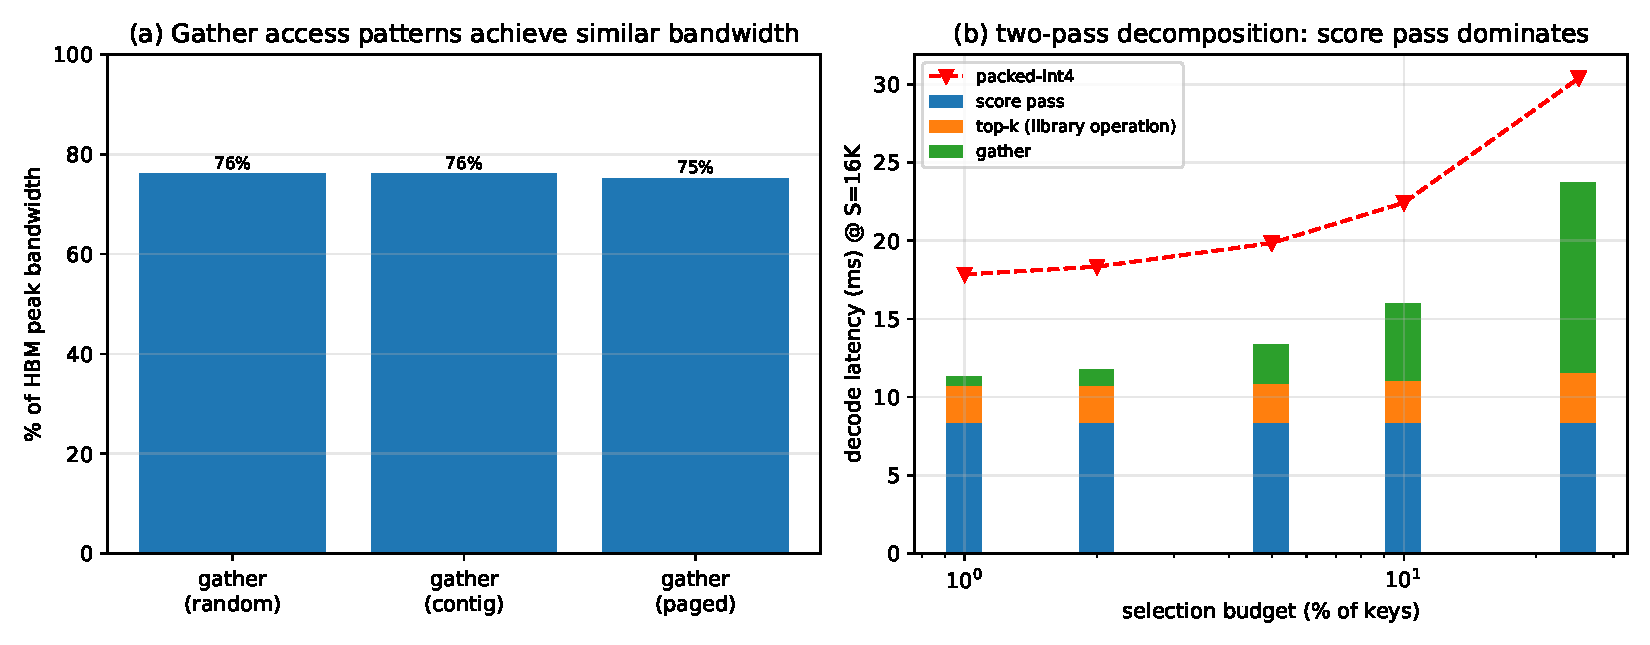
\includegraphics[width=0.96\textwidth]{fig_study_profiling.pdf}
\Description{Two panels on the RTX 4000 Ada. Panel (a) is a bar chart showing that
random, contiguous, and paged selected-value gather access patterns each achieve
about 75--76 percent of peak HBM bandwidth. Panel (b) is a stacked bar and line chart
decomposing sparse fp8 decode latency into score, top-k, and gather stages across
selection budgets, with an overlaid packed-int4 curve that is slower than fp8 at every
budget despite reading fewer nominal score bytes.}
\caption{Why byte count does not predict decode latency on the RTX~4000 Ada.
(a) The three selected-value gather access patterns achieve similar fractions of the
360\,GB/s peak; higher is better. (b) Sparse fp8 decode is decomposed into the
all-key score pass, top-$k$, and selected-value gather. The red dashed curve is the
measured packed-int4 path, which is slower despite smaller nominal score-key storage.}
\label{fig:profiling}
\end{figure*}

\begin{table}[t]
\centering\footnotesize\setlength{\tabcolsep}{4pt}
\caption{Decode latency at 16K context and batch 32. Lower is better. Sparse methods
use a 5\% retained-key budget and include scoring, top-$k$, and gather inside the
CUDA graph.}
\label{tab:latency}
\begin{tabular}{l r}
\toprule
method & decode latency (ms) \\
\midrule
KIVI-2 & 6.07 \\
two-pass sparse (fp8, $k{=}5\%$) & 7.31 \\
KIVI-4 & 7.78 \\
FP8 dense & 9.88 \\
BF16 dense & 12.63 \\
two-pass sparse (int2 score, $k{=}5\%$) & 13.01 \\
two-pass sparse (int4 score, $k{=}5\%$) & 19.85 \\
\bottomrule
\end{tabular}

\end{table}

\subsection{The latency crossover is a regime, not a universal ranking}
The full crossover grid resolves the scope of the 16K, 5\% profile. Figure~\ref{fig:crossover}
compares sparse fp8 decode against KIVI-2 at fixed large-model tensor shape. The
boundary moves with both context length and retained-key budget: sparse fp8 wins in
the low-budget cells, where avoiding value reads is useful, while KIVI-2 wins once
the retained set is sufficiently large that its compact stored cache and fused decode
path dominate. This is the systems point of the comparison. Neither ``sparse'' nor
``two-bit'' identifies the faster path without the operating point.

\begin{figure*}[t]
\centering
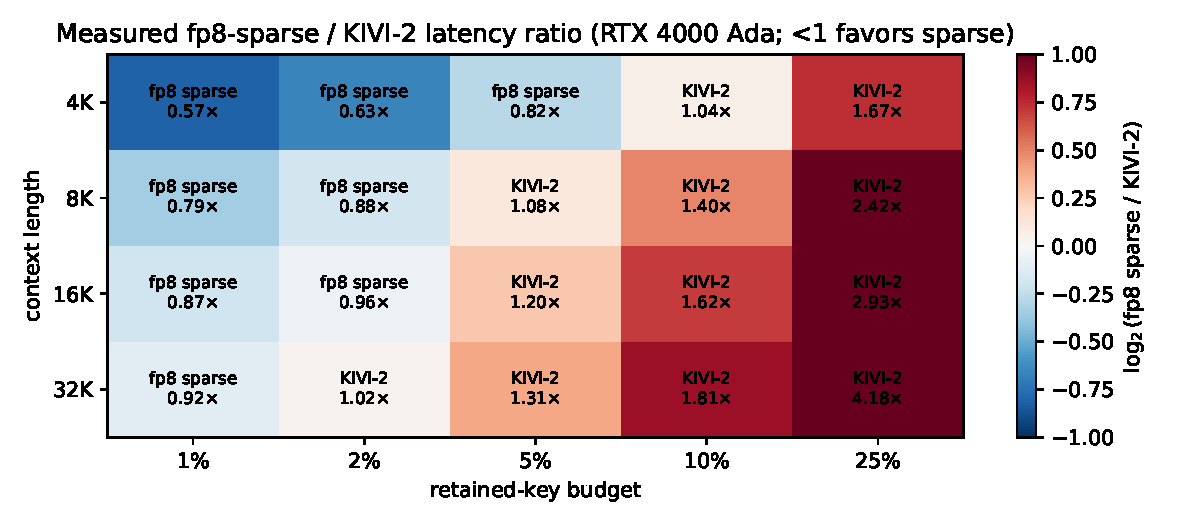
\includegraphics[width=0.78\textwidth]{fig_crossover_regimes.pdf}
\Description{A heatmap grid with context length (4K to 32K) on the vertical axis and
retained-key budget (1\% to 25\%) on the horizontal axis. Each cell reports whether
sparse fp8 or KIVI-2 decode is faster and the latency ratio. Sparse fp8 wins in the
low-budget, shorter-context cells (ratios as low as 0.57x), while KIVI-2 wins as
context length and retained-key budget grow (ratios up to 4.18x), showing the
crossover boundary shifts with both axes.}
\caption{Measured sparse-fp8 versus KIVI-2 decode crossover on the RTX~4000 Ada
($B{=}32$, $D{=}128$, $H_q/H_k{=}64/8$). Each cell shows the faster measured method
and the latency ratio. The complete 4--32K grid is shown; 64K is omitted because only
the 1\% sparse-fp8 cell completed within available memory. The boundary changes with
both context and retained-key budget.}
\label{fig:crossover}
\end{figure*}

The independent-capture measurements in Figure~\ref{fig:robustness} show that the
packed-score penalty is not an artifact of a single graph capture: at the 5\% slice,
the fp8, int4, and int2 paths retain their observed ordering across the two fully
reproducible full-decode contexts. The right panel of Figure~\ref{fig:robustness} separates a complementary issue. Changing head
dimension changes the absolute score work and the packed-to-fp8 ratio, so the kernel
finding should be read as a characterization of these shapes on Ada rather than as a
hardware-independent law. Together, the panels make the claim appropriately narrow:
the byte-count heuristic fails throughout the measured sweep, but its quantitative
crossover must be remeasured for a new architecture or serving kernel.

\begin{figure*}[t]
\centering
\begin{minipage}[t]{0.49\textwidth}
\centering
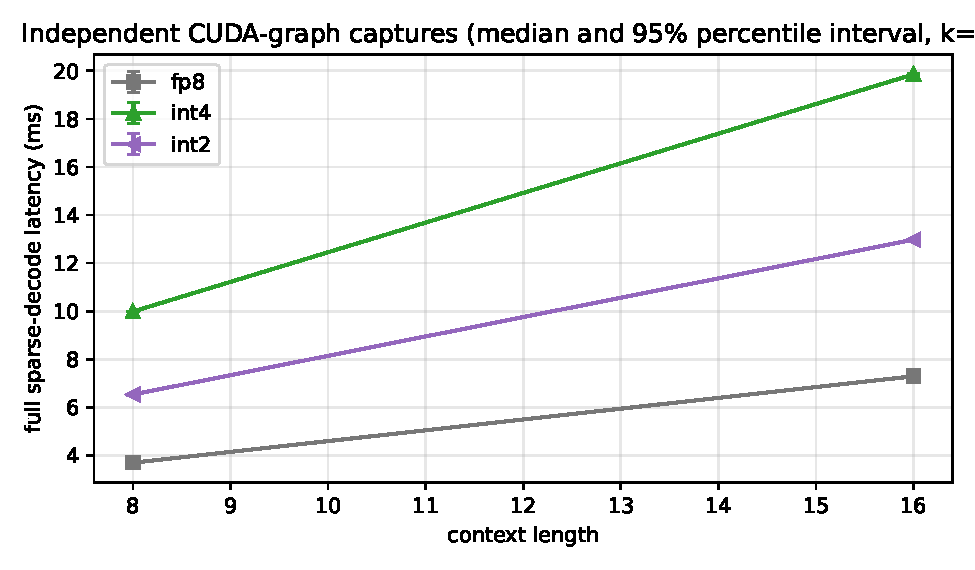
\includegraphics[width=\textwidth]{fig_latency_robustness.pdf}\\[-2pt]
\footnotesize (a) Complete sparse decode, independent captures
\end{minipage}\hfill
\begin{minipage}[t]{0.49\textwidth}
\centering
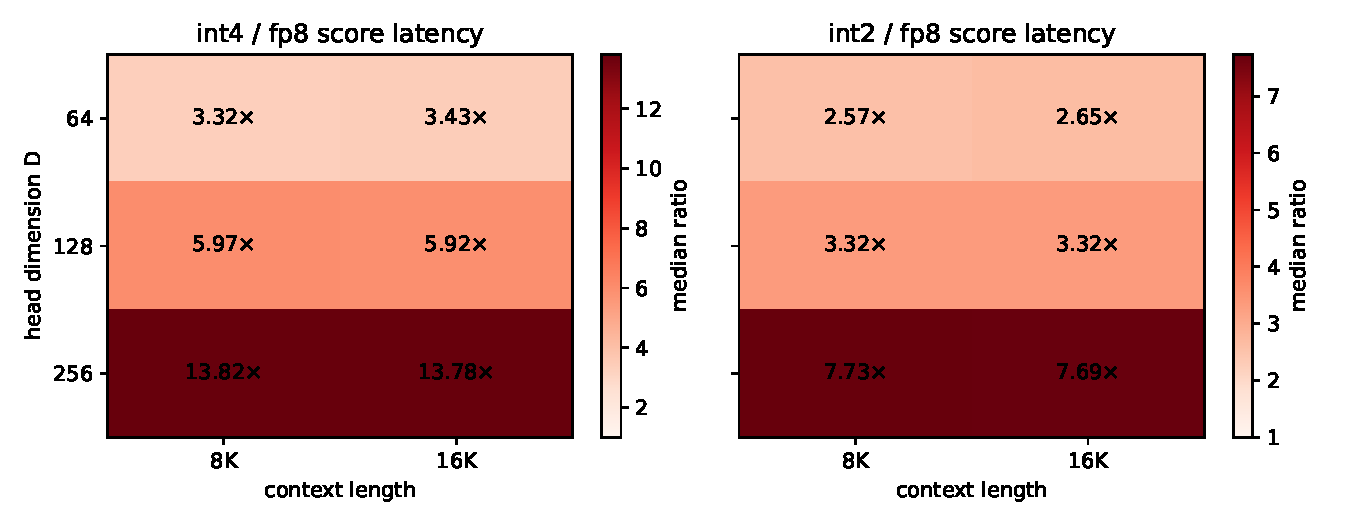
\includegraphics[width=\textwidth]{fig_score_shape_sweep.pdf}\\[-2pt]
\footnotesize (b) Score-kernel shape sweep
\end{minipage}
\Description{Two panels. Panel (a) is a line chart of full sparse-decode latency
versus context length (8K to 16K) for fp8, int4, and int2 scoring, plotted as medians
with 2.5th--97.5th percentile bands from 15 independently captured CUDA graphs; int4
is slowest, fp8 fastest, at every context length. Panel (b) is a pair of heatmaps
showing the median packed-score latency ratio (int4/fp8 and int2/fp8) over a sweep of
head dimension and context length, with ratios ranging from about 2.6x to 6x,
indicating packed low-bit scoring is consistently slower than fp8 across shapes.}
\caption{Robustness checks for the latency characterization. (a) Medians and 2.5th--
97.5th percentile ranges over 15 independently captured graphs, each timed over 100
replays, for the complete sparse path at $k{=}5\%$. (b) Median packed-score latency
relative to fp8 over the context/head-dimension sweep. Both panels use the same
RTX~4000 Ada and grouped-query shape as the main profile.}
\label{fig:robustness}
\end{figure*}

\subsection{Observed panels and the resource tradeoff}
The additional observed panels are consistent with the main selection pattern, but do
not establish universal stability. On Qwen2.5-1.5B/3B and Llama-3.2-3B, fp8 tracks
the exact-key oracle closely in the reported cells; PQ-LUT and int4 are also close at
the same scoring cost in most panels, while the tested page selection and eviction
implementations are worse at low budgets. PG19 and the 8K/32K panels show the same
qualitative separation in the observed windows. At the 7B 8K scale-transfer point,
fp8, PQ-LUT, and int4 are within 0.04 PPL of the exact selector at both measured
budgets; Quest is 9.23 PPL at 1\% versus a 5.64 dense reference. The released
per-window observations and intervals support these scoped descriptions.

Table~\ref{tab:transfer} gives a compact view at the 5\% operating point. Absolute
PPL is not comparable across rows because the models differ, so the table is useful
for the within-column relationship: across the displayed configurations, the fp8,
PQ-LUT, and int4 values remain near the exact-key reference, whereas the tested Quest
implementation is farther away. The Qwen2.5-7B column is the preregistered 8K
fallback after the 16K run exceeded available memory; it is a scale-transfer point,
not a claim about larger models or all contexts.

\begin{table}[!ht]
\centering\footnotesize
\caption{Selection transfer at a 5\% budget. PPL is shown separately for each
model/context; compare methods within a column, not absolute values across columns.
Q0.5B/Q1.5B/Q3B are Qwen2.5 at 16K, L3B is Llama-3.2-3B at 16K, and
$^\dagger$Q7B is Qwen2.5-7B at the preregistered 8K fallback.}
\label{tab:transfer}
\begin{tabular}{l r r r r r}
\toprule
selector ($k{=}5\%$) & Q0.5B & Q1.5B & Q3B & L3B & Q7B$^\dagger$ \\
\midrule
dense & 9.17 & 6.72 & 5.89 & 5.79 & 5.64 \\
exact-key & 9.30 & 6.78 & 5.94 & 6.00 & 5.66 \\
fp8 scalar & 9.29 & 6.78 & 5.94 & 6.00 & 5.64 \\
PQ-LUT & 9.31 & 6.78 & 5.94 & 6.00 & 5.66 \\
int4 scalar & 9.34 & 6.82 & 5.95 & 6.02 & 5.63 \\
Quest (page) & 9.99 & 7.45 & 11.31 & 12.93 & 5.95 \\
\bottomrule
\end{tabular}

\end{table}

The 7B NIAH panel supplies an independent scale-transfer check that is not reducible
to average language-model loss. It retains the hard 8-token recent window, 100 paired
needle placements, and the 1--2\% budgets where granularity is most consequential.
Table~\ref{tab:niah_transfer} therefore asks a precise question: at the available 8K
7B setting, do the per-key score representations retain the rare relevant token as
often as the exact-key ranking reference, and does the page-level implementation
show the same qualitative limitation? The answer is reported with paired-case
intervals rather than inferred from the small-model panel.

\begin{table}[t]
\centering\footnotesize
\caption{Hard NIAH scale-transfer panel (Qwen2.5-7B, 8K, recent window 8): retrieval
rate with 95\% paired bootstrap intervals over 100 cases. This is a 7B validation at
the available context, not a claim of general downstream-task coverage.}
\label{tab:niah_transfer}
\begin{tabular}{l c c}
\toprule
selector & $k{=}1\%$ & $k{=}2\%$ \\
\midrule
exact & 1.00 [0.96,1.00] & 1.00 [0.96,1.00] \\
PQ-LUT & 1.00 [0.96,1.00] & 1.00 [0.96,1.00] \\
int4 scalar & 0.96 [0.90,0.98] & 1.00 [0.96,1.00] \\
Quest & 0.32 [0.24,0.42] & 0.86 [0.78,0.91] \\
\bottomrule
\end{tabular}

\end{table}

% ==================================================================

\begin{table*}[t]
\centering\small
\caption{Capacity and one selection--compression composition point
(Qwen2.5-0.5B, Wikitext-2 for PPL). Left: maximum decode batch on the 20\,GB GPU.
Right: selection and attention representations at the same 5\% budget.}
\label{tab:capacity_compose}
\begin{tabular}{l r r}
\toprule
method & $S{=}16$K & $S{=}32$K \\
\midrule
BF16 & 128 & 64 \\
FP8 & 256 & 128 \\
KIVI-4 & 256 & 128 \\
Sparse-INT2 & 32 & 16 \\
\bottomrule
\end{tabular}
\hspace{1.4cm}
\begin{tabular}{l r}
\toprule
selection / attend cache & PPL @ $k{=}5\%$ \\
\midrule
exact / bf16 & 9.30 \\
exact / fp8 & 9.53 \\
fp8 / bf16 & 9.29 \\
fp8 / fp8 & 9.41 \\
\bottomrule
\end{tabular}

\end{table*}



Compression and selection nevertheless optimize different resources. In the 20\,GB
capacity experiment, KIVI-4 supports batches of 256 and 128 at 16K and 32K contexts,
whereas Sparse-INT2 supports 16 at both lengths because it retains a high-precision
attention cache plus a score representation. Selection reduces value traffic; it does
not automatically reduce storage. The two mechanisms can be composed: at a 5\%
budget, combining fp8 selection with an fp8 attention cache yields 9.41 PPL, no worse
than the attention-compression penalty alone within this experiment. These results
support a staged design: compress for capacity, select for traffic, and measure the
combined kernel path.

Table~\ref{tab:capacity_compose} shows why these are not substitute axes. KIVI-4 and
FP8 convert smaller stored representations directly into batch headroom. Sparse-INT2
instead retains an attention cache plus a score representation, so its selective read
savings do not become a capacity saving. The composition panel isolates a different
question: changing the attend cache from bf16 to FP8 moves the 5\% PPL from 9.29--9.30
to 9.41--9.53, while changing the selector at a fixed attend cache changes little in
this panel. Thus composition is plausible and useful, but it must be measured rather
than inferred from the isolated axes.


% ==================================================================
\section{Design Implications}
The experiments suggest a compact reporting contract for KV-cache systems. Quality
comparisons should state key storage, value storage, scoring representation,
accumulation precision, selection unit, recent window, and retained-key budget.
Performance comparisons should separate score, ranking, gather, and attention time
instead of converting nominal bytes directly into latency. Capacity should be
reported independently because a sparse method may retain more state than a dense
quantized cache. These fields are not bookkeeping details: each one changes a ranking
observed in this study.

The same separation guides implementation. A compact score code is useful only if
its GPU kernel retains the expected bandwidth advantage. A page index is useful only
if the saved metadata compensates for its coarser selection unit. A low-precision
oracle is useful only if its top-$k$ agreement survives the model's key distribution.
The deployable operating point is therefore not the representation with the fewest
bits, but the composition whose storage, selection, and attention stages all remain
in favorable regimes.


% ==================================================================
\section{Limitations}
Quality is measured on Qwen2.5 from 0.5B to 7B and Llama-3.2-3B using Wikitext-2,
PG19, perplexity, and synthetic retrieval; it does not establish behavior on 14B+
models or a full downstream task suite. The Qwen2.5-7B sparse evaluation exceeded
available memory at 16K, so we use the preregistered 8K fallback and release the OOM
record. Gemma-2 is excluded because the selection hook does not reproduce its logit
soft-capping and sliding-window attention exactly.

The latency study characterizes one RTX~4000 Ada operating point using synthetic
large-model attention shapes. This is sufficient to establish the measured
bottleneck transition on that architecture, but other architectures and end-to-end
serving stacks may place the crossover elsewhere. H2O, SnapKV, and Quest are
controlled implementations of their core mechanisms rather than the original
systems' fully tuned stacks. The 16-bit accumulation failure is observed on the one
evaluated model that exposes it. Key-channel clipping does not by itself repair the
bf16 failure, so the general recommendation is to validate the oracle, not to assume
a single outlier mechanism or that every model fails in the same way.

% ==================================================================
\section{Conclusion}
KV-cache efficiency cannot be inferred from bits per token or retained-key percentage
alone. In the matched experiments, value representation has the larger observed PPL
effect in the compression ablation, selection granularity creates the largest observed
sparse-quality separation, and scalar int4 is competitive with a product-quantized
scoring code at the same byte cost. At the measured Ada point, the packed
reconstruction path makes low-bit scoring slower despite smaller nominal score-key
storage; low-precision accumulation can also corrupt the ranking oracle itself. A
useful KV-cache design must therefore separately measure storage, scoring, selection,
and attention before composing their savings.

\section*{\acksname}
Generative AI tools were used in preparing and editing portions of the manuscript and
research artifact. The authors verified the final text, code, reported results, and independently arrived at all conclusions.

\bibliographystyle{ACM-Reference-Format}
\bibliography{references}

\end{document}
